\documentclass{article}
\usepackage{tikz}
\usetikzlibrary{calc}
\begin{document}
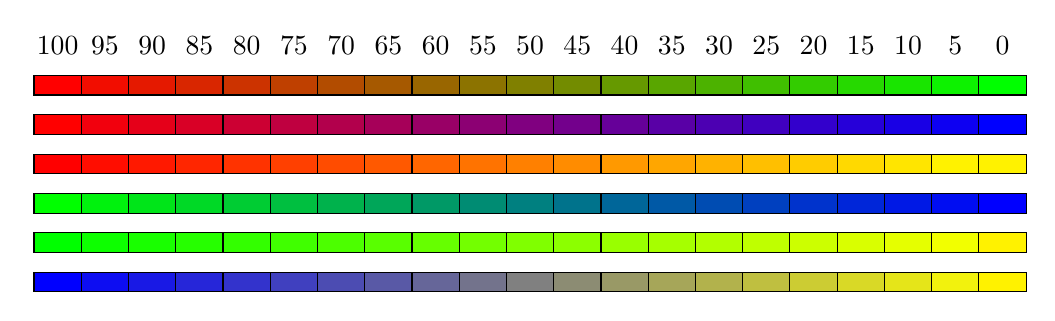
\begin{tikzpicture}[x=6mm, y=2.5mm]
\foreach \m in {100,95,...,0}
{
	\coordinate (A) at ($ (0,2) + 0.2*(100-\m,0) $);
	\coordinate (B) at ($ (1,3) + 0.2*(100-\m,0) $);
	\node at ($ (A)!0.5!(B) $) {\m};
}
\foreach \x in {100,95,...,0}
{
	\coordinate (A) at ($ (0,0) + 0.2*(100-\x,0) $);
	\coordinate (B) at ($ (1,1) + 0.2*(100-\x,0) $);
	\filldraw[fill=red!\x!green] (A) rectangle (B);
}
\foreach \x in {100,95,...,0}
{
	\coordinate (A) at ($ (0,-2) + 0.2*(100-\x,0) $);
	\coordinate (B) at ($ (1,-1) + 0.2*(100-\x,0) $);
	\filldraw[fill=red!\x!blue] (A) rectangle (B);
}
\foreach \x in {100,95,...,0}
{
	\coordinate (A) at ($ (0,-4) + 0.2*(100-\x,0) $);
	\coordinate (B) at ($ (1,-3) + 0.2*(100-\x,0) $);
	\filldraw[fill=red!\x!yellow] (A) rectangle (B);
}
\foreach \x in {100,95,...,0}
{
	\coordinate (A) at ($ (0,-6) + 0.2*(100-\x,0) $);
	\coordinate (B) at ($ (1,-5) + 0.2*(100-\x,0) $);
	\filldraw[fill=green!\x!blue] (A) rectangle (B);
}
\foreach \x in {100,95,...,0}
{
	\coordinate (A) at ($ (0,-8) + 0.2*(100-\x,0) $);
	\coordinate (B) at ($ (1,-7) + 0.2*(100-\x,0) $);
	\filldraw[fill=green!\x!yellow] (A) rectangle (B);
}
\foreach \x in {100,95,...,0}
{
	\coordinate (A) at ($ (0,-10) + 0.2*(100-\x,0) $);
	\coordinate (B) at ($ (1,-9) + 0.2*(100-\x,0) $);
	\filldraw[fill=blue!\x!yellow] (A) rectangle (B);
}
\end{tikzpicture}
\end{document}
